Designing your own data types means that your code can work with more meaningful values. You can design the data that is stored in the program so that it is organised in ways that will help make the processing simpler.

\subsection{Designing Small DB} % (fold)
\label{sub:designing_small_db}

\tref{tbl:small-db-prog} contains a description of the Small DB program that will be explored in this chapter. This is a small program that will read, store, and output values entered by the user.

\begin{table}[h]
\centering
\begin{tabular}{l|p{10cm}}
  \hline
  \multicolumn{2}{c}{\textbf{Program Description}} \\
  \hline
  \textbf{Name} & \emph{Small DB} \\
  \\
  \textbf{Description} & Reads text (up to 7 characters), integer, and double values from the user, storing them within the program and then outputting their values to the Terminal along with the type being stored in the program. Each value will be stored in a row with a unique identifier that will be assigned by the system. The first value will be assigned the id 0, the second will be assigned the id 1, and so on.\\
  \hline
\end{tabular}
\caption{Description of the Small DB program.}
\label{tbl:small-db-prog}
\end{table}

As before, the process to design and implement this program will follow a number of steps:
\begin{enumerate}
  \item Understand the problem, and get some ideas on the tasks that need to be performed.
  \item Choose the artefacts we will create and use
  \item Design the control flow for the procedural\footnote{The Program, and any Functions and Procedures.} artefacts
  \item Map these artefacts to code
  \item Compile and run the program
\end{enumerate}

% subsection designing_small_db (end)

\subsection{Understanding Small DB} % (fold)
\label{sub:understanding_small_db}

This program does not perform any complex functionality, so it does not require much analysis to understand the tasks that need to be performed.

Data identified:
\begin{itemize}
  \item \textbf{Row}: has a unique identifier, and a value.
  \item \textbf{Column Value}: each value in a row is either an integer, a double, or a text value.
\end{itemize}

Tasks to be performed:
\begin{itemize}
  \item \textbf{Read Row}: The program needs to be able to read a row from the user.
  \item \textbf{Print Row}: After reading the value the program need to output the value to the Terminal.
\end{itemize}

% subsection understanding_small_db (end)
\clearpage
\subsection{Choosing Artefacts for Small DB} % (fold)
\label{sub:choosing_artefacts_for_small_db}

The process of choosing the artefacts for a program involves determining both the structure of the data, as well as the structure of the functions and procedures. In many cases the structure of the data is more important than the structure of the functionality, as getting the data right will make the processing easier. Therefore, the first task is to consider how the data can be structured.

The three main tools that you have for designing the structure of the data in your program are \textbf{records}, \textbf{unions}, and \textbf{enumerations}. A record allows you to create a composite data type that is made up of a number of fields. The union allows you to create a type that stores one kind of data, or another. Finally the enumeration allows you to create a list of available options.

\subsubsection{Looking for records in Small DB} % (fold)
\label{ssub:looking_for_records_in_small_db}

The most common of these is the \textbf{record}, a \textbf{struct} in C. This type allows you to create a single composite value that is composed of a number of related field values. This can be used to model the \emph{entities} in your program. When designing with records you think about the things you want to model, and the data associated with these things.

In the case of the Small DB program there appears to be one kind of record: the \texttt{row}. The program needs to store \textbf{row} values, where each row has a unique id (an integer), and a data value. These two values \emph{together} make up a row.

This data type will also work nicely with the planned functionality for the program. The code needs to be able to read and print \texttt{row} values. This means that this code can accept/return \texttt{row} values. The \texttt{Print Row} procedure will take in a \texttt{row} parameter, and print out its details to the \texttt{Terminal}. The \texttt{Read Row} function can read values from the user and return a \texttt{row} value to the caller.

% subsubsection looking_for_records_in_small_db (end)

\subsubsection{Looking for unions in Small DB} % (fold)
\label{ssub:looking_for_unions_in_small_db}

The \textbf{union}\footnote{\textbf{Variant record} in Pascal} is going to be less common than records, but they can offer some useful flexibility when designing your code. The union gives you the ability to have a type that stores one of a selection of types. If your program requires the ability to store different types at the one location then a union is a useful way of modelling this.

Reading the description of the Small DB program there does appear to be the need for a union. Each \texttt{row} needs to be able to store \emph{either} a Integer, a Double, or a text value. Using a union it will be possible to create a type to model this. This can be called the \texttt{Column Value} type, and will be the union of these three values.

The great thing about a union is that it stores only one value, the one that you assign to it. This means that it takes only the size needed to store the largest kind of value. In our case the \texttt{Column Value} will need space to store an Integer (4 bytes), a Double (8 bytes), or 7 Characters (8 bytes, 7 + 1 overhead). This will only need \textbf{8 bytes} of space, as at any one time it can only have one of these values. 

% subsubsection looking_for_unions_in_small_db (end)

\subsubsection{Looking for enumerations in Small DB} % (fold)
\label{ssub:looking_for_enumerations_in_small_db}

The last type to look for is the enumeration. This can be used to code a list of available options. Reading through the description of the program there is no really obvious list of options, but on further analysis there may be.

Remember that the Union does not know which value you stored in it. So you would be able to store a value in a Row, but then you would not know which value to read back from the union. This is where an enumeration can come in handy. You can create an enumeration that gives options for each of the kinds of values that the union can store. In this case the options can be \texttt{INT\_VAL}, \texttt{DBL\_VAL}, and \texttt{TXT\_VAL}, and can be called \texttt{Data Kind}.

The \texttt{Data Kind} enumeration allows you to declare variables that will have one of the available options as its value. This value will need to be stored for each \texttt{Row} in the program, so a field needs to be added to the \texttt{Row} type. This \texttt{kind} field can then store a marker that indicates the kind if value that is stored in the record.

This is a common pattern you will find for working with unions. It is called a \textbf{tagged union}. The enumeration value is the \textbf{tag} and stores an indicator of the kind of value stored in the union. This is the model behind the implementation of unions in Pascal, but must be manually coded in C.

% subsubsection looking_for_enumerations_in_small_db (end)

\subsubsection{Overall data design} % (fold)
\label{ssub:overall_data_design}

\tref{tbl:dd-small-db} shows the structures chosen for the data Small DB program. These provide the data model that will be used by the code to implement the program's logic. Having planned out the structure for the data of this program, the next step will be to design its logic.

\begin{table}[htbp]
  \centering
  \begin{tabular}{|l|l|l|}
    \hline
    \textbf{Data} & \multicolumn{2}{c|}{\textbf{Details}}  \\ 
    \hline
    \multicolumn{3}{c}{} \\
    \hline
    \textbf{\texttt{Row}} & \multicolumn{2}{l|}{A \textbf{record/struct} with the following fields:}  \\
    \hline
    & \texttt{id} & An \textbf{Integer} value that stores the unique id. \\
    \hline
    & \texttt{kind} & A \textbf{Data Kind} value indicating the type of data being stored in this record. \\
    \hline
    & \texttt{data} & Stores \textbf{Column Value} data containing the actual data. \\ 
    \hline
    \multicolumn{3}{c}{} \\
    \hline
    \textbf{\texttt{Data Kind}} & \multicolumn{2}{l|}{A \textbf{enumeration} with the following options:}\\
    \hline
    & \texttt{INT\_VAL} & Indicates the row is storing an Integer value. \\
    \hline
    & \texttt{DBL\_VAL} & Indicates that the row is storing a Double value. \\
    \hline
    &  \texttt{TXT\_VAL} & Indicates that the row is storing a text value. \\
    \hline
    \multicolumn{3}{c}{} \\
    \hline
    \textbf{\texttt{Column Value}} & \multicolumn{2}{l|}{A \textbf{union} that stores one of the following:}\\
    \hline
    & \texttt{Int Val} & An Integer value. \\
    \hline 
    & \texttt{Dbl Val} & A Double value. \\
    \hline
    & \texttt{Txt Val} & A text value, with up to seven characters. \\
    \hline
  \end{tabular}
  \caption{Data Dictionary for Small DB}
  \label{tbl:dd-small-db}
\end{table}

% subsubsection overall_data_design (end)

\subsubsection{Reading a Row} % (fold)
\label{ssub:reading_a_row}

The first piece of functionality to implement can be the \texttt{Read Row} function. This function will be responsible for reading a value from the user, and determining if that value is an integer, double, or string and then storing it in the row with the correct tag value.

To implement this will require the ability to check if the value in a string is an integer or a double. These two tasks can be coded into functions \texttt{Is Integer} and \texttt{Is Double}. Other than this the remaining code just needs to copy values into the fields of the \texttt{Row} that will be returned.

\texttt{Read Row} will need to accept a single parameter, \texttt{Next Id}. This will be the value assigned to the \texttt{id} field of the \texttt{Row}, and will be passed in as this data will be managed elsewhere. At the end of the function, \texttt{Read Row} will return a single \texttt{Row} value. As this is a \textbf{record}, it will contain \texttt{id}, \texttt{kind}, and \texttt{data} values.

\begin{figure}[p]
   \centering
   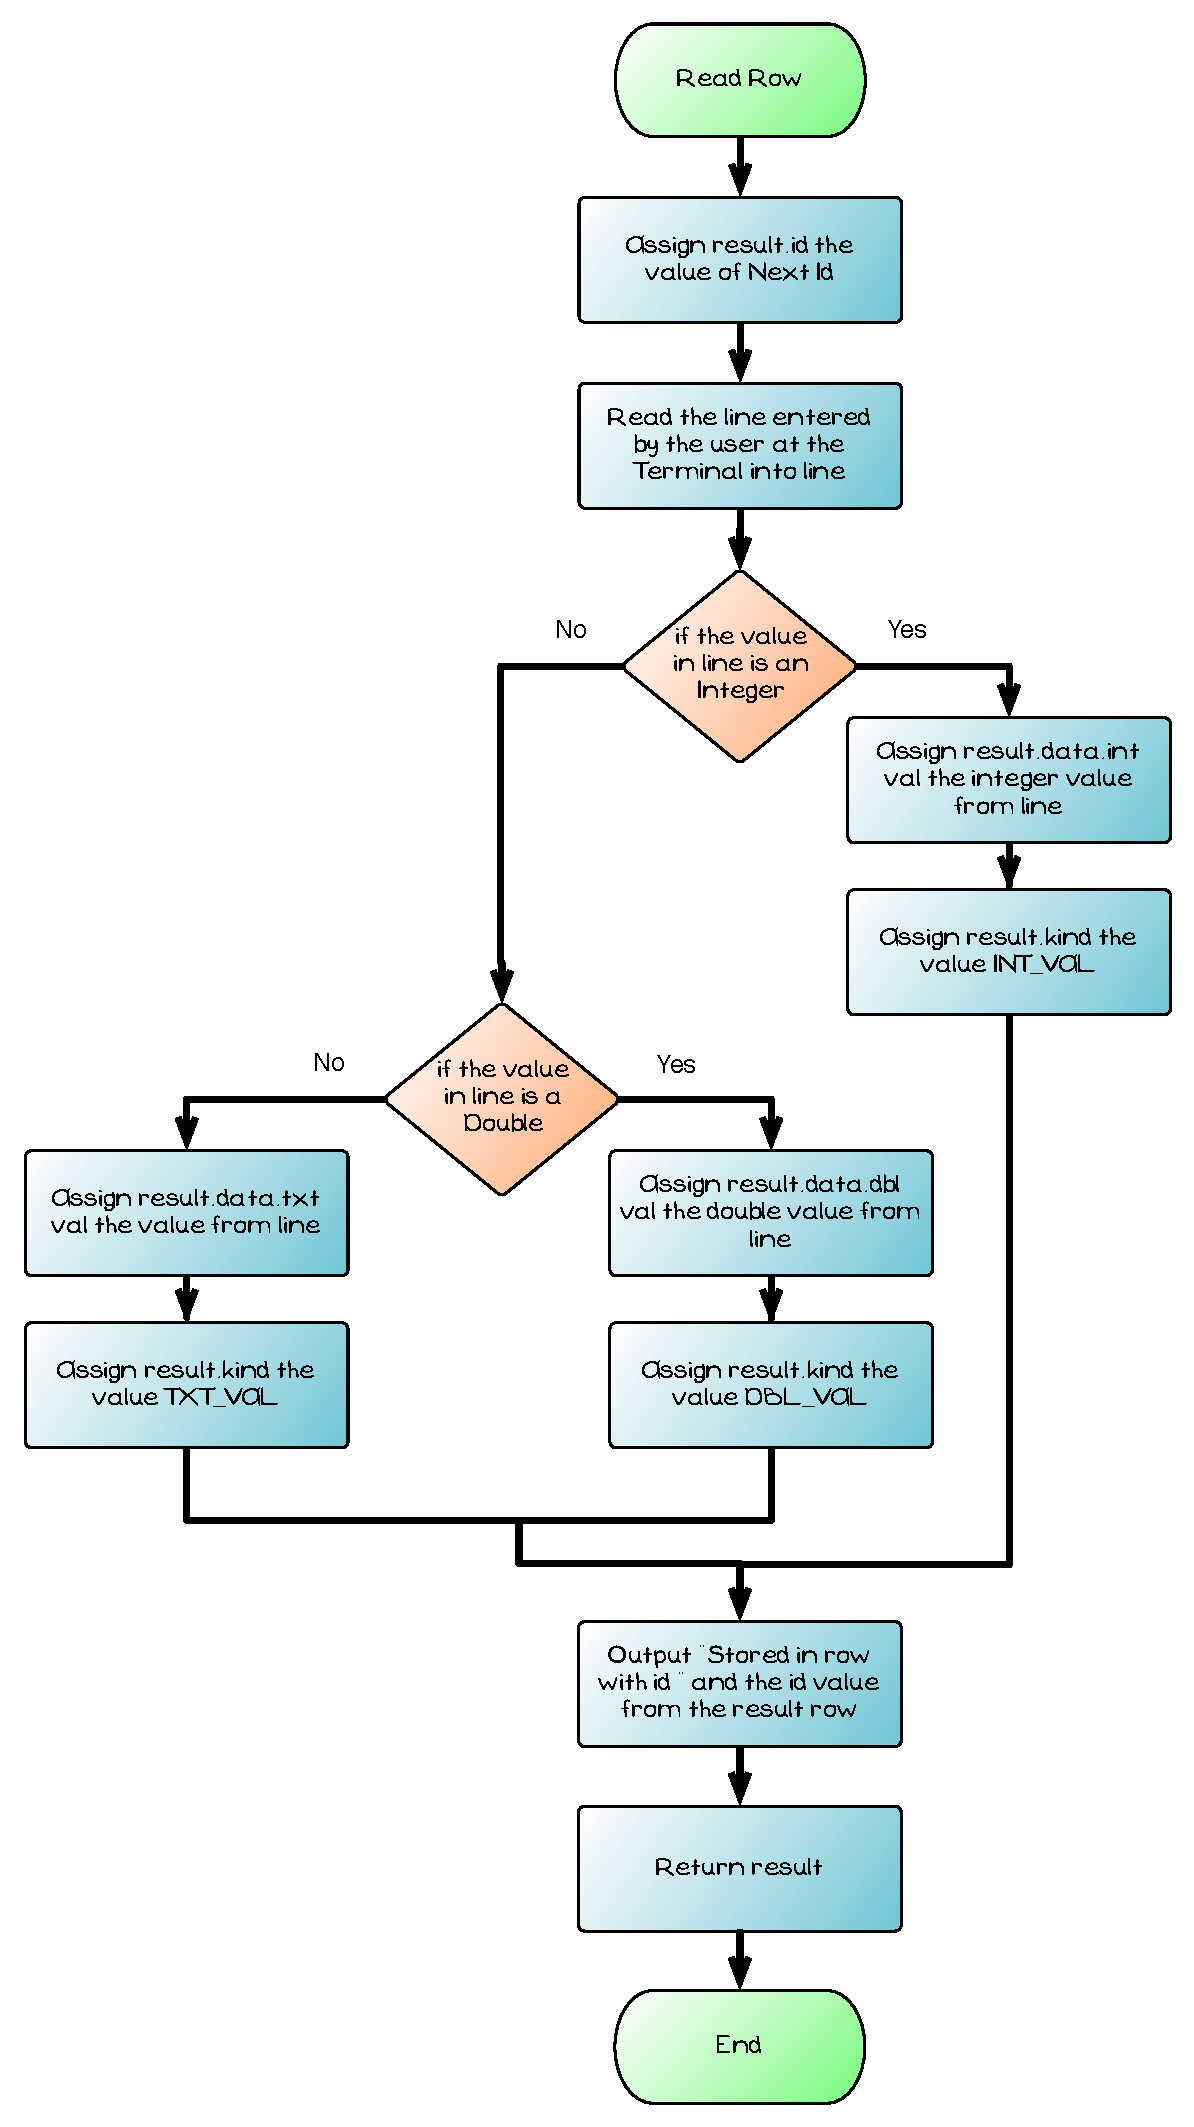
\includegraphics[width=0.80\textwidth]{./topics/type-decl/diagrams/ReadRowFlow} 
   \caption{Flowchart for \texttt{Read Row}}
   \label{fig:read-row-flow}
\end{figure}

\fref{fig:read-row-flow} shows the flowchart for the steps in the \texttt{Read Row} function. Notice that all three fields of the \texttt{Row} are assigned values. The \texttt{id} is assigned in the first statement, whereas the \texttt{data} and \texttt{kind} fields are assigned values in the branches of the if statements. All of this data is then returned when the result value is returned.

The \textbf{union} is being used when the \texttt{data} field is assigned a value. When the \emph{integer} branch is taken the union is assigned a value via its \texttt{int val} field. When the \emph{double} branch is taken the union is assigned a value via its \texttt{dbl val} field. When neither of these branches is taken, the \emph{text} value is assigned to the union via its \texttt{txt val} field.

Finally, one of the options from the \textbf{enumeration} is stored in the \texttt{kind} field of the record alongside the union's value. This means that the \texttt{INT\_VAL} value is stored in the \texttt{kind} field when the \emph{integer} branch is taken, and the \texttt{DBL\_VAL} value is stored when the \emph{double} branch is taken, and the \texttt{TXT\_VAL} value is stored when the \emph{text} path is taken.

\fref{fig:read-row-data} shows three examples of the kinds of values that could be the \texttt{result} of this function when it returns. In each case there are three field values in the row. These are defined in the \texttt{Row} record, and include the \texttt{id}, the \texttt{kind}, and the \texttt{data}.

\begin{figure}[htbp]
   \centering
   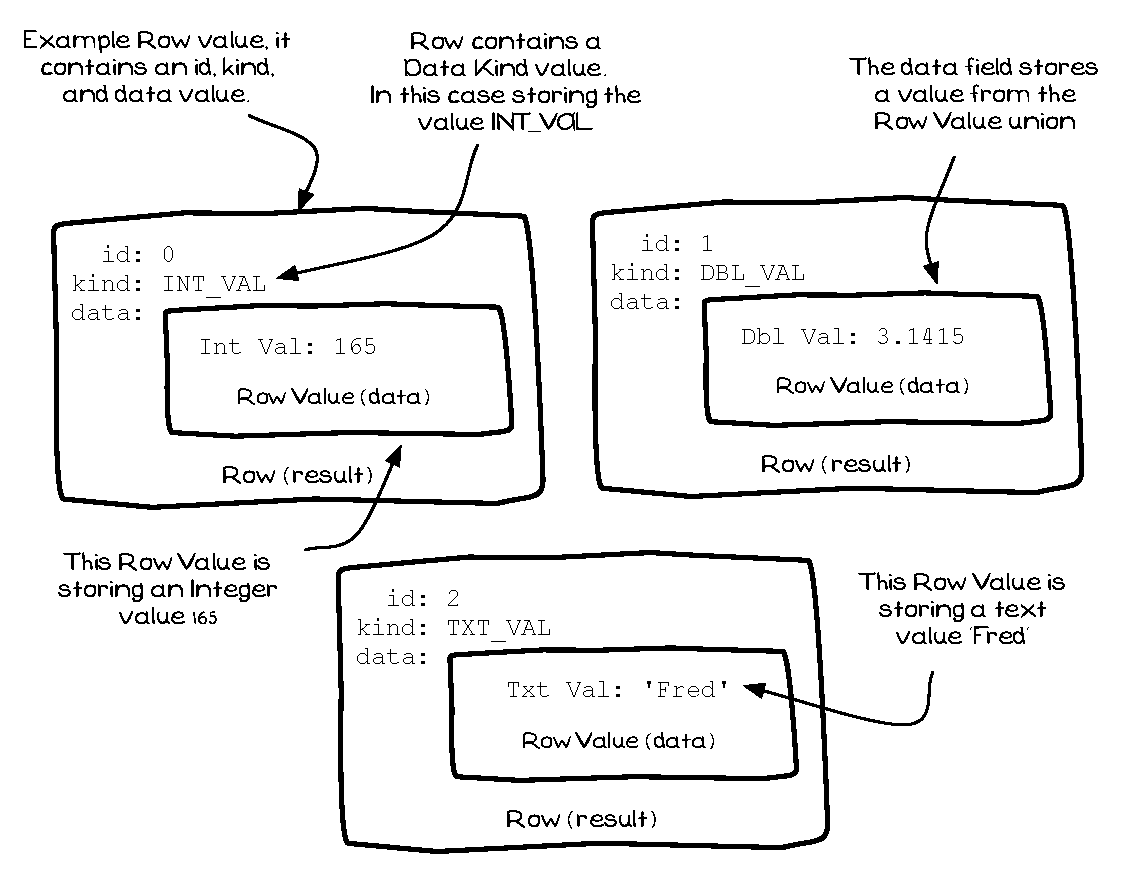
\includegraphics[width=0.8\textwidth]{./topics/type-decl/diagrams/RowDataRead} 
   \caption{Examples of data that could be read into a \texttt{Row} value in \texttt{Read Row}}
   \label{fig:read-row-data}
\end{figure}

% subsubsection reading_a_row (end)
\clearpage
\subsubsection{Printing a Row} % (fold)
\label{ssub:printing_a_row}

Having read data into a \texttt{Row} it is now possible to output that to the Terminal. The steps required to do this can be coded into a \texttt{Print Row} procedure. The required steps are shown in the flowchart in \fref{fig:print-row-flow}.

The \texttt{Print Row} procedure will take a single \texttt{Row} parameter. This parameter will contain the data related of the row that is to be output to the Terminal. The procedure will output the \texttt{id} value and the \texttt{data} values from the \texttt{Row}, using the \texttt{kind} value to determine which field to access from the \texttt{Column Value} union.

The \texttt{row}'s \texttt{id} can be output straight away as it is an Integer value. The actual data that needs to be output depends on the kind of value that is stored in the \texttt{Row}. A \nameref{sub:case_statement} can be used to select a path based upon the value stored in the row's \texttt{kind} field. The four paths here cater for the three options from the \texttt{Data Kind} enumeration, plus an additional path in case the value in \texttt{To Print}'s \texttt{kind} field does not match\footnote{A enumeration is stored as an Integer value, meaning it is possible to store other values in here.} one of these. This path would indicate a bug in the software, but should be included just to be safe.

\begin{figure}[htbp]
   \centering
   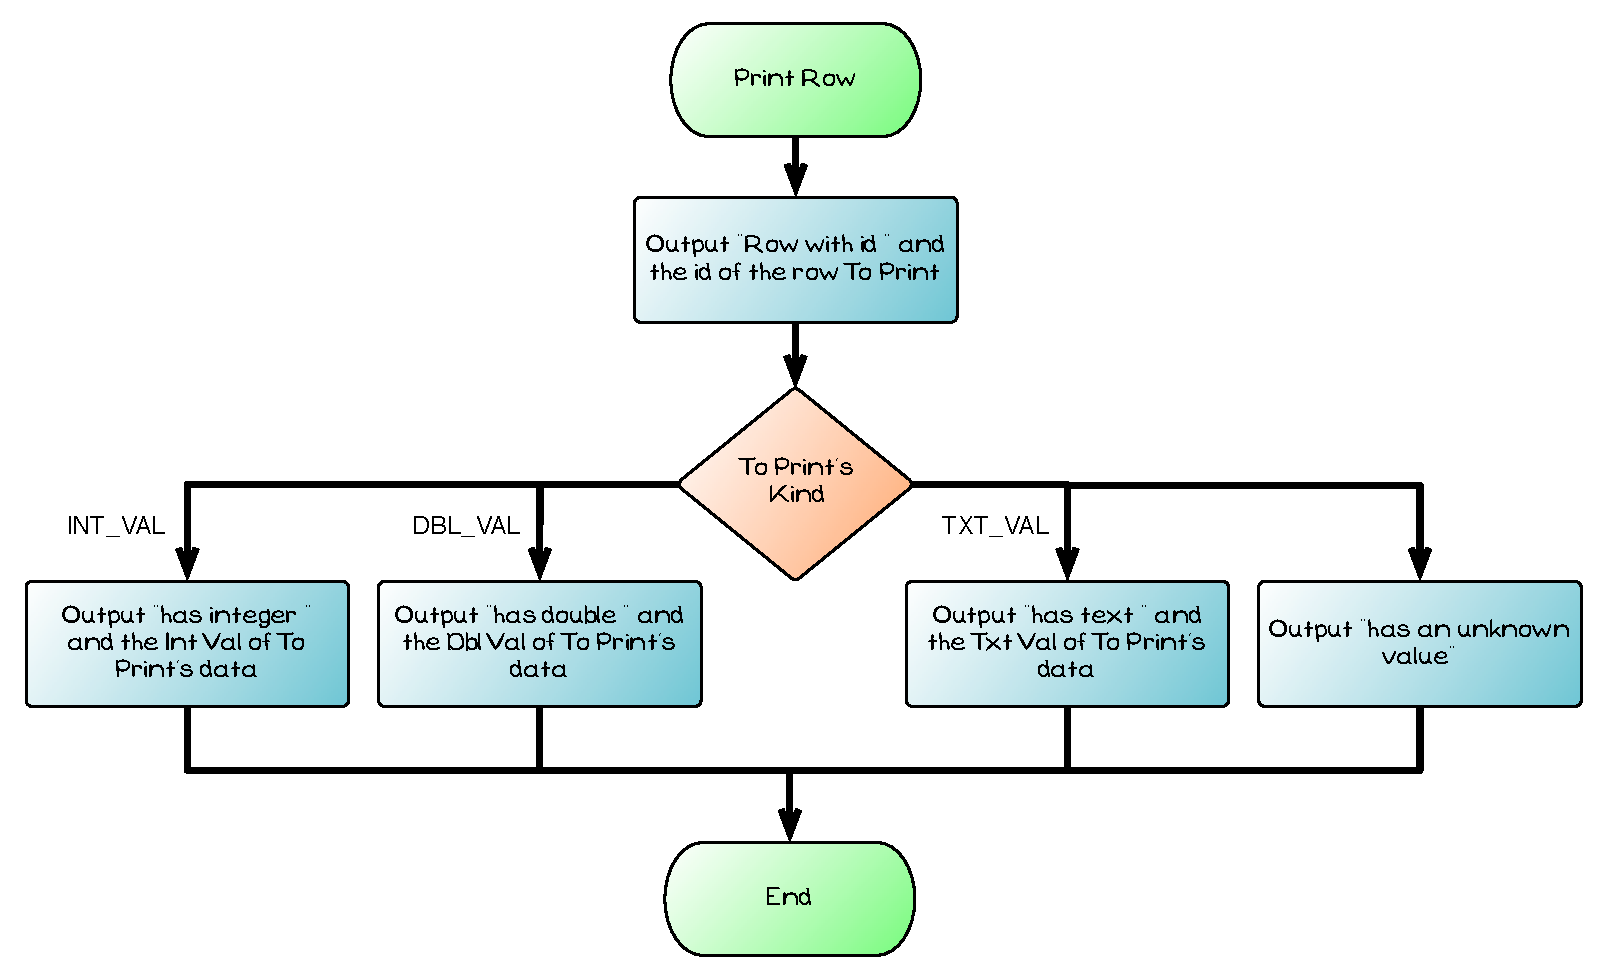
\includegraphics[width=\textwidth]{./topics/type-decl/diagrams/PrintRowFlow} 
   \caption{Flowchart of the steps needed to print a \texttt{Row} to the Terminal}
   \label{fig:print-row-flow}
\end{figure}

% subsubsection printing_a_row (end)
\clearpage
\subsubsection{Overview of Small DB's design} % (fold)
\label{ssub:overview_of_small_db_s_design}

\fref{fig:small-db-struct} shows the structure chart for the design of the Small DB program. The functionality is split between the \texttt{Read Row} function and the \texttt{Print Row} procedure, with \texttt{Is Integer} and \texttt{Is Double} providing useful utility functions to test the data read from the user.

\begin{figure}[htbp]
   \centering
   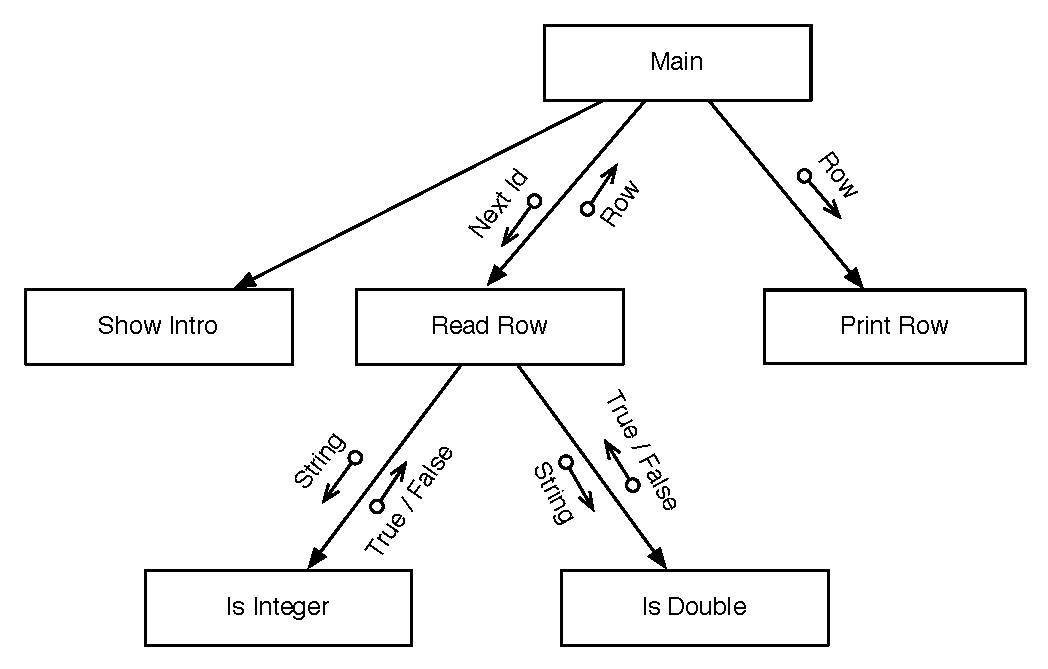
\includegraphics[width=0.85\textwidth]{./topics/type-decl/diagrams/SmallDBStruct} 
   \caption{Structure chart showing the overview of the Small DB program}
   \label{fig:small-db-struct}
\end{figure}

The \texttt{Main} procedure will be responsible for storing the data read from the user in an \nameref{sub:array} of \texttt{Row} values. The logic in \texttt{Main} will then loop over this array once to read in a value \emph{for each} element of the array, using \texttt{Read Row} to get this value. \texttt{Main} with then loop over the array a second time, this time calling \texttt{Print Row} \emph{for each} element in the array. This will allow \texttt{Main} to read in, and then print out, all of the rows.

A \texttt{Show Intro} procedure has also been added to this design to house the code to show the startup message to the user. This moves this code out of the \texttt{main} procedure allowing it to focus on coordinating the tasks involved in working with the array of \texttt{Row} values.

% subsubsection overview_of_small_db_s_design (end)
% subsubsection choosing_artefacts_for_small_db (end)

\subsection{Writing the Code for Small DB} % (fold)
\label{sub:writing_the_code_for_small_db}

The flowcharts and Pseudocode shown communicate the logic that needs to be coded into the Functions and Procedures of this Program. The following two sections, \sref{sec:custom_types_in_c} \nameref{sec:custom_types_in_c} and  \sref{sec:custom_types_in_pascal} \nameref{sec:custom_types_in_pascal}, contain a description of the syntax needed to code your own types in the C and Pascal programming languages. This information can be used to write the code for the Small DB program, and others.

% subsection writing_the_code_for_small_db (end)

\clearpage
\subsection{Compiling and Running Small DB} % (fold)
\label{sub:compiling_and_running_small_db}

Remember to code and run this one small piece after the other. For this you could start by writing the \texttt{Print Row} procedure, and pass it values that you hard code in the program. This will allow you to experiment with storing different values in the fields of the record and union without having to deal with the user input and testing functions. You can test this by checking that the output matches what you expect based on the values in the \texttt{Row}.

Once this is complete the next task would be to work on the \texttt{Read Row} function, and its helpers. These have a bit more logic and will require that you test it more carefully. Think about the kind of test data that you can use to check each of the paths through these functions, and use this to check your code as you progress.

\fref{fig:small-db-using} shows the program in operation.

\begin{figure}[h]
   \centering
   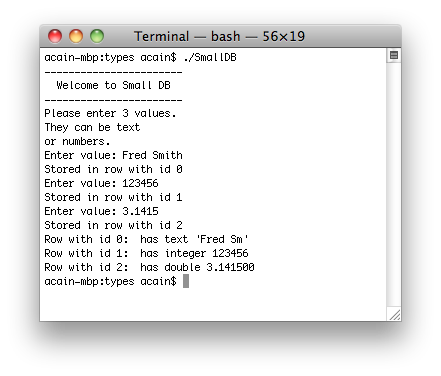
\includegraphics[width=0.9\textwidth]{./topics/type-decl/images/SmallDB} 
   \caption{Small DB run from the Terminal, repeated from \fref{fig:small-db}}
   \label{fig:small-db-using}
\end{figure}


% subsection compiling_and_running_small_db (end)
